\specsection{2.1 Сформулировать определение случайной величины и функции распределения вероятностей
случайной величины. Доказать свойства функции распределения}

\OPR Случайной величиной называют функцию $X:\Omega\rightarrow\mathbb{R}$, такую, что для $\forall x\in\mathbb{R}$ мн-во $\{\omega : X(\omega)<x\}\in \beta$ (т.е. это мн-во является событием)

\OPR Функцией распределения (вероятностей) случ. величины $X$ называется отображение $F:\mathbb{R}\rightarrow\mathbb{R}$, определённое условием $F(x) = P\{X<x\}$

Свойства функции распределения
\begin{enumerate}[topsep=0pt, leftmargin=20pt, noitemsep, label=\arabic*\degree]
	\item $0\leq F(x) \leq 1$
	
	\item если $x_1\leq x_2$, то $F(x_1)\leq F(x_2)$, т.е. $F(x)$ неубывающая ф-ия.
	
	\item $\liml_{\toinf[-]{x}}F(x) = 0,~~\liml_{\toinf[+]{x}}F(x) = 1$
	
	\item $P\{x_1\leq x<x_2\}=F(x_2)-F(x_1)$
	
	\item $\liml_{x\rightarrow x_0}F(x)=F(x_0)$, т.е. $F(x)$ непрерывна слева в каждой точке $x\in\mathbb{R}$
	
	\item [] Доказательства
	
	\setcounter{enumi}{0}
	
	\item $F(x)=P\{X<x\}\Rightarrow0\leq F(x)\leq 1$
	
	\item $\mathbb{A}_1=\{X<x_1\}, \mathbb{A}_2=\{X<x_2\}$
	\item [] т.к. $x_1\leq x_2$, то $\mathbb{A}_1\subseteq \mathbb{A}_2$. По свойству вер-ти $P(A_1)\leq P(A_2),~F(x_1)\leq F(x_2)$
	
	\item $\liml_{\toinf[+]{x}}=1$. 
	\item [] рассмотрим последовательность $x_1,...,x_n,..$ такую, что
	\item [] 1) $x_1\leq x_2\leq x_3\leq ...\leq x_n\leq...$. ~ 2) $x_n\rightarrow+\infty$ при $n\rightarrow\infty$
	\item [] рассмотрим последовательность событий  $\mathbb{A}_n=\{X<x_n\},~n\geq 1$
	\item [] тогда $A_n,~n=1,2,...$ -- возраст. т.к. $\mathbb{A}_i\subseteq\mathbb{A}_{i+1},~i=1,2,...$
	\item [] в соотв. с аксиомой непрерывности $\lim P\{\mathbb{A}_n\}=P\{\bigcup\limits_{n=1}^{\infty} \mathbb{A}_{n}\}=P\underbrace{\{X<+\infty\}}_{\text{достов. событие}}=1$
	\item [] т.к. $P\{\mathbb{A}_n\}=P\{X<x_n\}=F(x_n)$, то $\liml_{\toinf[+]{x}}F(x_n)=1$
	\item [] т.к. $x_n$ - произвольная последоват., то в соотв. с опред. предела ф-ии по Гейне
	\item [] $\liml_{\toinf[+]{x}}F(x)=1$. ~ $\liml_{\toinf[-]{x}}F(x)=0$ доказывается аналогично

	\item ~
	\item []
	\begin{minipage}{\linewidth}
		\centering
		\begin{minipage}{0.25\linewidth}
				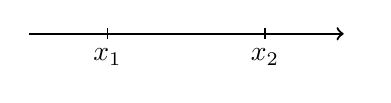
\begin{tikzpicture}
				\draw[thick,->] (0,0) -- (4,0) node[anchor=north west] {};
				\draw (1,2pt) -- (1,-2pt) node[anchor=north] {$x_1$};
				\draw (3,2pt) -- (3,-2pt) node[anchor=north] {$x_2$};
			\end{tikzpicture}
			\item []
			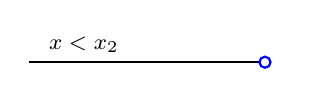
\begin{tikzpicture}
				\draw[thick,-] (0,0) -- (2.95,0) node[anchor=north west] {};
				\node[above] at (0.7,0) {\footnotesize{$x < x_2$}};
				\draw[blue,thick] (3,0) circle (2pt);
			\end{tikzpicture}
			\item []
			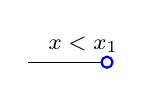
\begin{tikzpicture}
				\draw[thin,-] (0,0) -- (0.95,0) node[anchor=north west] {};
				\node[above] at (0.7,0) {\footnotesize{$x < x_1$}};
				\draw[blue,thick] (1,0) circle (2pt);
			\end{tikzpicture}
			\item []
			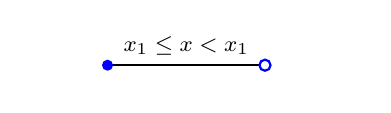
\begin{tikzpicture}
				\draw[white,thick,-] (0,0) -- (4,0) node[anchor=north west] {};
				\draw[thick,-] (1.05,0) -- (2.95,0) node[anchor=north west] {};
				\node[above] at (2,0) {\footnotesize{$x_1\leq x < x_1$}};
				\fill[blue,thick] (1,0) circle (2pt);
				\draw[blue,thick] (3,0) circle (2pt);
			\end{tikzpicture}
		\end{minipage}
		\hspace{0.05\linewidth}
		\begin{minipage}{0.65\linewidth}
			$\{X<x_2\}=\{X<x_1\}+\{x_1\leq X < x_2\}$ -- события в объединении несовместные
			
			$\Rightarrow \underbrace{P\{X<x_2\}}_{F(B)}=\underbrace{P\{X<x_1\}}_{F(A)}+P\{x_1\leq X<x_2\}$
			
			$\Rightarrow P\{x_1\leq X<x_2\}=F(x_2)-F(x_1)$
		\end{minipage}
	\end{minipage}
	
	\item Рассмотрим посл-ть $x_1,...,x_n,...$ к-я 1) $x_1\leq x_2\leq...\leq x_n\leq...<x_0$ ~ 2) $x_n\rightarrow x_0$
	\item [] тогда $\mathbb{A}_n=\{X<x_n\}$ -- неубыв. посл. событий
	\item [] $\liml_{n\rightarrow\infty}F(x)=\liml_{n\rightarrow\infty}P\{A_n\}\stackrel{\text{акс. непрер.}}{=}P\{\bigcup\limits_{n=1}^{\infty}\mathbb{A}_n\}=P\{X<x_0\}=F(x_0)$
	\item [] По опред. предела ф-ии по Гейне: $\liml_{x\rightarrow x_0-}F(x)=F(x_0)$
\end{enumerate}


\clearpage
